\documentclass{article}
\usepackage{amsfonts, amsmath, amssymb, amsthm} % Math notations imported
\usepackage{enumitem}
\usepackage{graphicx}
\usepackage{setspace}
\usepackage{indentfirst}
\usepackage[margin=1in]{geometry}
\graphicspath{{./images/}} % Path to images

% \begin{figure}[htb!]
%      \centering
%      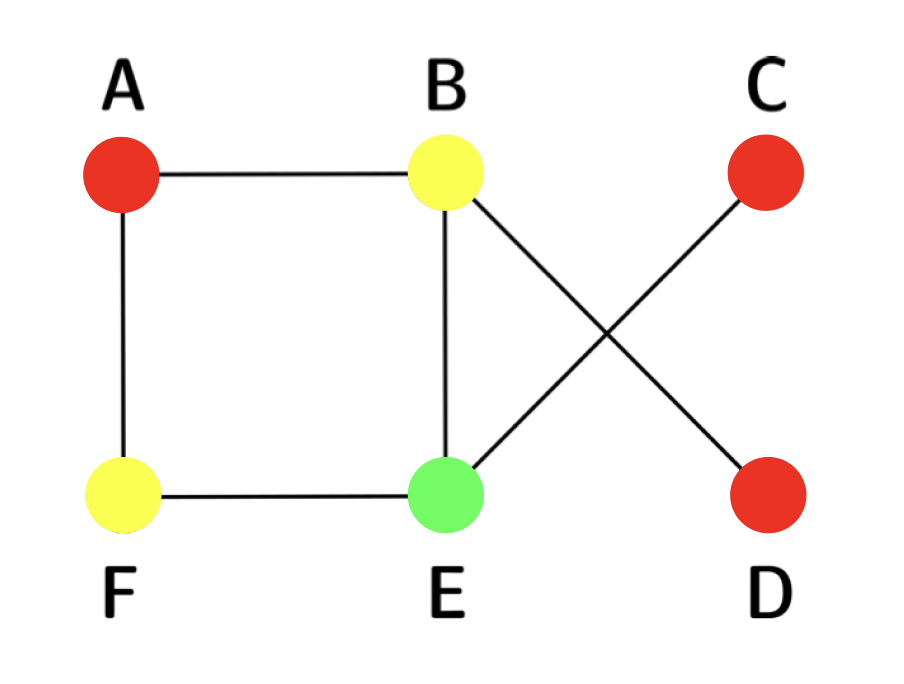
\includegraphics[scale=0.5]{coloring.png}
%      \caption{Coloring of the graph.}
% \end{figure}

% \begin{figure}[htb]
%     \qquad
%     \begin{minipage}{.4\textwidth}
%         \centering
%         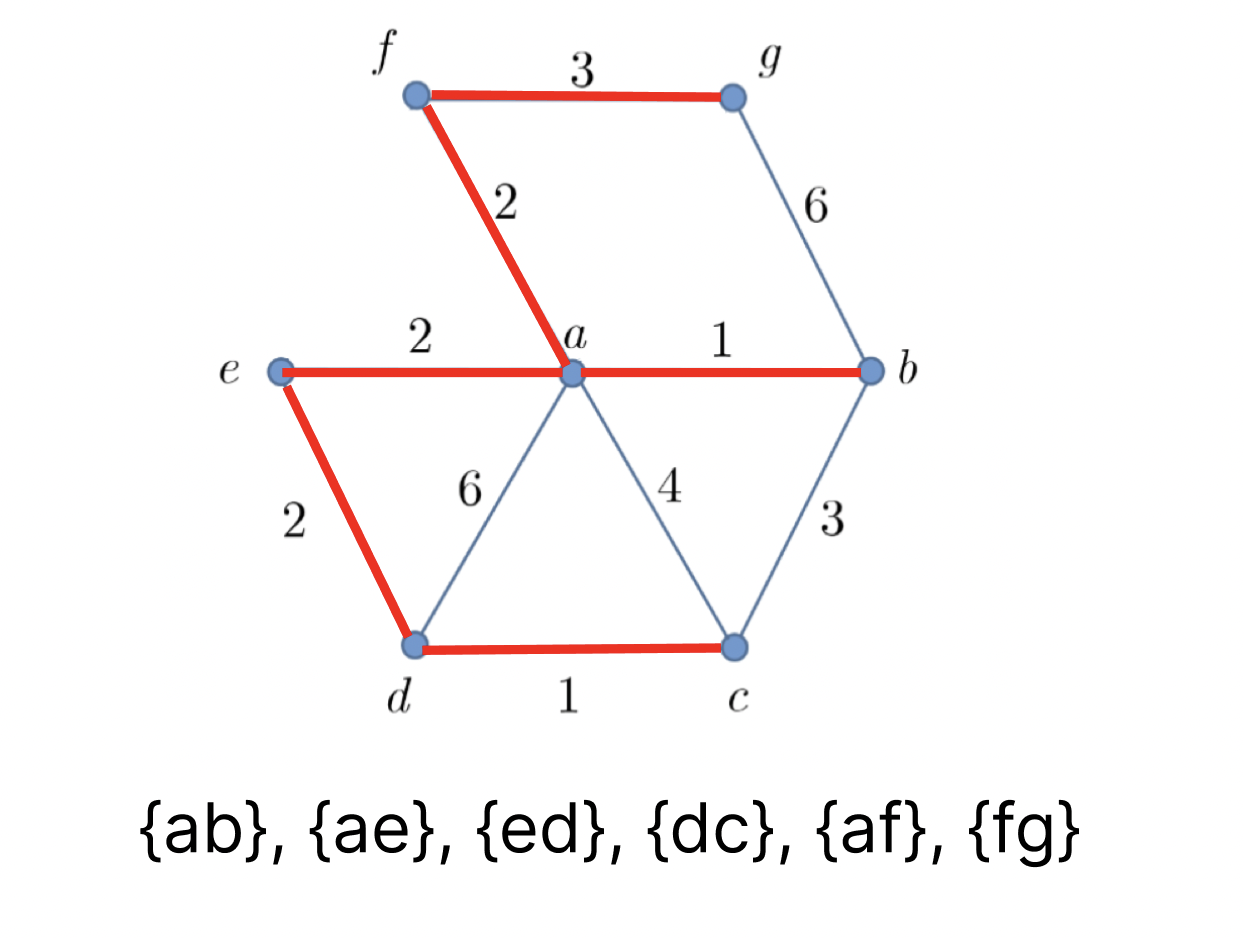
\includegraphics[scale=0.35]{prims.png}
%         \caption{}
%     \end{minipage}    
%     \qquad
%     \begin{minipage}{.4\textwidth}
%         \centering
%         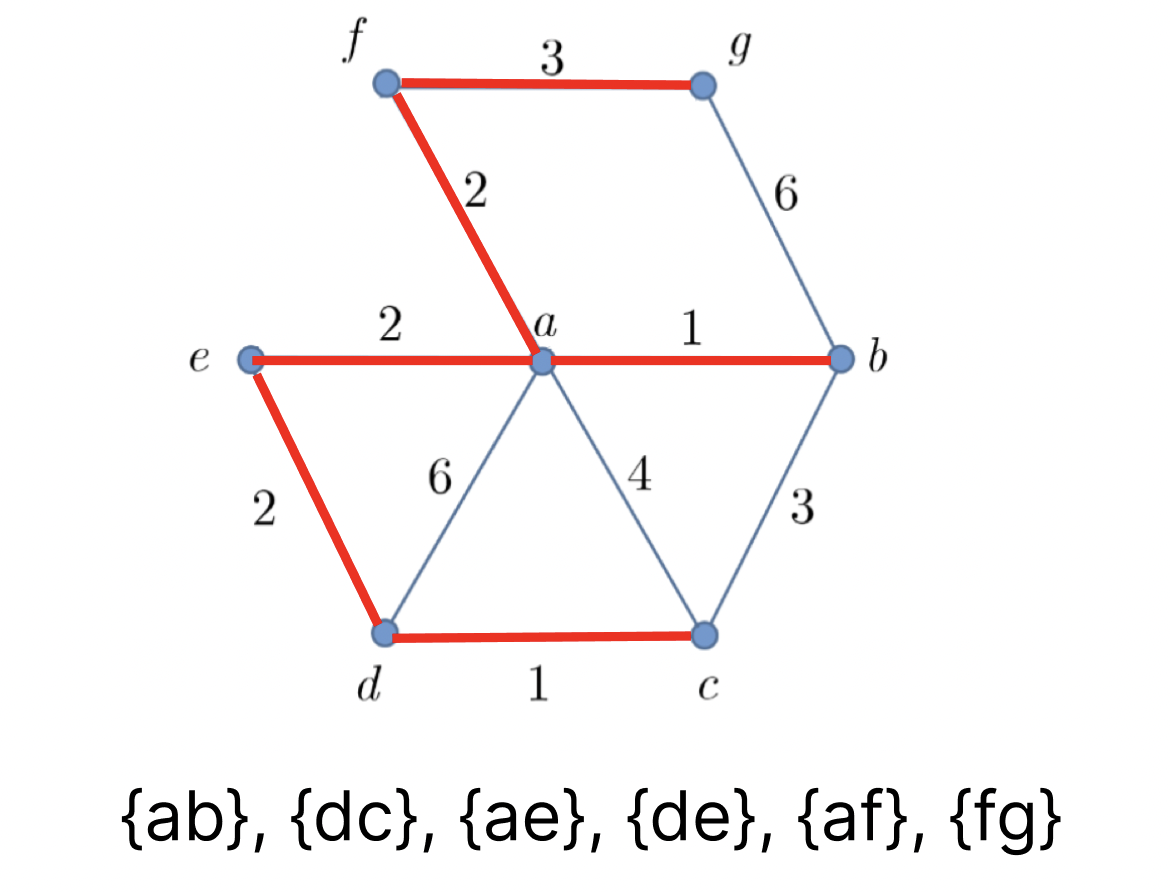
\includegraphics[scale=0.35]{kruskal.png}
%         \caption{}
%     \end{minipage}        
% \end{figure} 

\newtheorem{thm}{Theorem}
\newtheorem{proposition}[thm]{Proposition}
\newtheorem{cor}[thm]{Corollary}

% title information
\title{Math 104 HW6}
\author{Neo Lee}
\date{10/13/2023}

\setstretch{1.15}
% main content
\begin{document} 

% placing title information; comment out if using fancyhdr
\maketitle 

\subsection*{Exercise 12.10}
\begin{proposition}
    $(s_n)$ is bounded if and only if $\lim \sup|s_n|<+\infty$.
\end{proposition}
\begin{proof}
    Forward direction: Suppose $(s_n)$ is bounded. Then there exists $M>0$ such that $|s_n|\leq M$ 
    for all $n\in\mathbb{N}$. Then $\sup|s_n|\leq M$, so $\lim\sup|s_n|\leq M<+\infty$ [recall 
    we have proved previously that a sequence $(t_n)\le M$ cannot have $\lim t_n>M$].

    Backward direction: Suppose $\lim\sup|s_n|<+\infty$. Then let $\lim \sup|s_n|=L$. By definition 
    of limit, there exists $N$ such that for all $n> N$, $|s_n|\le \sup |s_n|<L+1$. Then let 
    $M=\max\{|s_1|,|s_2|,\dots,|s_{N-1}|,|s_N|,L+1\}$. Then for all $n\in\mathbb{N}$, $|s_n|\leq M$, 
    so $(s_n)$ is bounded.
\end{proof}

\subsection*{Exercise 14.3}
Determine which of the following series converge:

\noindent \textbf{(a)} $\sum\frac{1}{\sqrt{n!}}$\quad \textbf{(b)} $\sum\frac{2+\cos n}{3^n}$
\quad \textbf{(c)} $\sum\frac{1}{2^n+n}$\quad \textbf{(d)} $\sum\left(\frac{1}{2}\right)^n
\left(50+\frac{2}{n}\right)$ \quad \textbf{(e)} $\sum\sin \left(\frac{n\pi}{9}\right)$ 
\quad \textbf{(f)} $\sum\frac{(100)^n}{n!}$.
\begin{proof}[Solution]\indent
    \begin{enumerate}[label=(\alph*)]
        \item Ratio Test:
        \begin{align*}
            \lim\sup\left|\frac{1}{\sqrt{(n+1)!}}\cdot\frac{\sqrt{n!}}{1}\right| & = \lim\sup\left|\frac{1}{\sqrt{n}}\right| \\
            & = \lim\left|\frac{1}{\sqrt{n}}\right| \\
            & = 0 < 1.
        \end{align*}
        So the series converges.

        \item Root Test:
        \begin{align*}
            \lim\sup\left|\frac{2+\cos n}{3^n}\right|^{\frac{1}{n}} & = \lim\sup\left|\frac{(2+\cos n)^{1/n}}{3}\right| \\
            & \le \lim\sup \left|\frac{(2+1)^{1/n}}{3}\right| \\
            & = \lim \left|\frac{3^{1/n}}{3}\right| \\
            & = \frac{1}{3} < 1.
        \end{align*}
        So the series converges.

        \item Comparison Test:
        Consider the series $\sum\frac{1}{2^n}$. Then for all $n\in\mathbb{N}$,
        \begin{align*}
            \left|\frac{1}{2^n+n}\right| \le \frac{1}{2^n}.
        \end{align*}
        We know that $\sum\frac{1}{2^n}$ converges by Root Test with 
        $\lim \left|\frac{1}{2^n}\right|^{1/n}=\frac{1}{2}$, so by comparison test, 
        $\sum\frac{1}{2^n+n}$ converges.

        \item Comparison Test:
        Consider the series $\sum\left(\frac{1}{2}\right)^n\cdot(52)$. Then for all $n\in\mathbb{N}$,
        \begin{align*}
            \left|\left(\frac{1}{2}\right)^n\left(50+\frac{2}{n}\right)\right| \le \left(\frac{1}{2}\right)^n\cdot(52).
        \end{align*}
        We know the series $\sum\left(\frac{1}{2}\right)^n\cdot(52)$ converges by Ratio Test with 
        $\lim\left|\frac{\left(\frac{1}{2}\right)^{n+1}\cdot(52)}{\left(\frac{1}{2}\right)^n\cdot(52)}\right|=\frac{1}{2}<1$,
        so by comparison test, $\sum\left(\frac{1}{2}\right)^n\left(50+\frac{2}{n}\right)$ converges.
    
        \item Consider $n_k = 9k+1$ and $n_j = 9k+2$ for all $k\in\mathbb{N}$. 
        Then $\sin\left(\frac{n_k\pi}{9}\right)$ and $\sin\left(\frac{n_j\pi}{9}\right)$ are two 
        different constant subsequences of $\sin\left(\frac{n\pi}{9}\right)$ with different limits,
        so $\sin\left(\frac{n\pi}{9}\right)$ diverges. In particular, it does not converge to $0$,
        so the series $\sum\sin\left(\frac{n\pi}{9}\right)$ diverges.

        \item Ratio Test:
        \begin{align*}
            \lim\sup\left|\frac{(100)^{n+1}}{(n+1)!}\cdot\frac{n!}{(100)^n}\right| & = \lim\sup\left|\frac{100}{n+1}\right| \\
            & = \lim \left|\frac{100}{n+1}\right| \\
            & = 0 < 1.
        \end{align*}
    \end{enumerate}
\end{proof}

\subsection*{Exercise 14.6}
\begin{enumerate}[label=(\alph*)]
    \item 
    \begin{proposition}
        If $\sum|a_n|$ converges and $(b_n)$ is a bounded sequence, then $\sum a_nb_n$ converges.
    \end{proposition}
    \begin{proof}
        We show that $\sum a_nb_n$ converges absolutely and hence converges. Since $(b_n)$ is bounded,
        there exists $M>0$ such that $|b_n|\le M$ for all $n\in\mathbb{N}$. Now notice
        \begin{align*}
            |a_nb_n| & = |a_n||b_n| \\
            & \le |a_n|M.
        \end{align*}
        Further, since $\sum |a_n|$ converges, $\sum |a_n|M = M\sum |a_n|$ also converges. Then by
        comparison test, $\sum |a_nb_n|$ converges, so $\sum a_nb_n$ converges absolutely.

        \emph{Alternatively,} since $(b_n)$ is bounded, we know there exists a $M'$ such that 
        $M' \ge |b_n|$ for all $n\in\mathbb{N}$. Now, denote
        $M = max\{M',1\}$. Then, we know there exists $N\in\mathbb{N}$ such that for $n\ge m>N$, 
        $\sum_{k=m}^n|a_k|<\frac{\epsilon}{M}$ for all $\epsilon>0$. Now, take such $N$ and
        \begin{align*}
            \sum_{k=m}^n|a_k| & < \frac{\epsilon}{M} \\
            M\sum_{k=m}^{n}|a_k| & < \epsilon \\
            \left|\sum_{k=m}^{n}a_kb_k\right| \le \sum_{k=m}^{n}|a_k||b_k| \le \sum_{k=m}^{n}|a_k|M & < \epsilon.
        \end{align*}
        Hence, $\sum a_nb_n$ satifies the Cauchy criterion and thus converges.
    \end{proof}

    \item Observe that \emph{Corollary 14.7}: absolute convergent series are convergent, is a 
    special case of (a).
    \begin{proof}[Solution]
        \emph{Corrollary 14.7} is a special case of (a) by taking $(b_n)=1$.
    \end{proof}
\end{enumerate}

\subsection*{Exercise 14.8}
\begin{proposition}
    If $\sum a_n$ and $\sum b_n$ are convergent series of nonnegative numbers, then 
    $\sum\sqrt{a_nb_n}$ converges. Hint: show $\sqrt{a_nb_n}\le a_n+b_n$ for all $n$.
\end{proposition}
Notice for all $n$
    \begin{align*}
        a_n^2 + b_n^2 + 2a_nb_n & \ge a_nb_n\\
        \left(a_n+b_n\right)^2 & \ge a_nb_n \\
        a_n + b_n & \ge \sqrt{a_nb_n}.
    \end{align*}

    Also, we know there exists $N_1$ such that for $n\ge m>N_1$, 
    $\left|\sum_{k=m}^na_k\right|<\epsilon/2$ and $N_2$ such that for $n\ge m>N_2$, 
    $\left|\sum_{k=m}^nb_k\right|<\epsilon/2$. Now we take $N = \max\{N_1,N_2\}$ for some 
    $\epsilon>0$. Then, for all $n\ge m>N$
    \begin{align*}
        \left|\sum_{k=m}^n\sqrt{a_nb_n}\right| & \le \left|\sum_{k=m}^{n}a_k+b_k\right| \\
        & \le \left|\sum_{k=m}^{n}a_k+\sum_{k=m}^{n}b_k\right| \\
        & \le \left|\sum_{k=m}^{n}a_k\right| + \left|\sum_{k=m}^{n}b_k\right| \\
        & < \epsilon.
    \end{align*}
    Hence, $\sum\sqrt{a_nb_n}$ satisfied Cauchy criterion and thus converges.
\subsection*{Exercise 14.9}
\begin{proposition}
    The convergence of a series does not depend on any finite number of terms, though the 
    value of the limit does. More precisely, consider series $\sum a_n$ and $\sum b_n$ and suppose 
    that the set $\{n\in\mathbb{N}:a_n\neq b_n\}$ is finite. Then the series both converge or else 
    the both diverge.
\end{proposition}
\begin{proof}
    Without loss of generality, we will focus on $\sum a_n$ and conclude the convergence of 
    $\sum b_n$ based on $\sum a_n$. Also, denote $M=\max\{n\in\mathbb{N}:a_n\neq b_n\}$.

    \underline{Case 1: $\sum a_n$ converges.} We know $\sum a_n$ satisfies Cauchy criterion, 
    thus we know there exists $N_1$ such that for all $n\ge m>N_1$, 
    $\left|\sum_{k=m}^{n}a_k\right|<\epsilon$ for some $\epsilon>0$. 
    
    Then, let 
    $N_2=\max\{N_1, M\}$. Since we have set $N_2$ to be at least $M$, any terms after $N_2$ for 
    $b_n$ is the same as $a_n$. Thus, any statement that holds true for $a_n$ is also true for $b_n$
    after $N_2$ and we can conclude for all $n\ge m>N_2$ $\left|\sum_{k=m}^{n}b_k\right|<\epsilon$ 
    for some $\epsilon>0$.

    Therefore, $\sum b_n$ satifies Cauchy criterion too and thus converges.

    \underline{Case 2: $\sum a_n$ diverges.} Assume for the sake of contradiction that $\sum b_n$ 
    converges. Then there exists $N_2$ for all $\epsilon>0$ such that for $n\ge m>N_2$, 
    $\left|\sum b_n\right|<\epsilon$. Thus, we can take $N_1=\max\{N_2,M\}$, which will make sure 
    that for $n\ge m>N_1$, $\left|\sum_{k=m}^n a_n\right|<\epsilon$. 
    But that contradicts that fact that $\sum a_n$ diverges. Hence, $\sum b_n$ must diverge.
\end{proof}

\subsection*{Exercise 14.14}
\begin{proposition}
    Show that $\sum_{n=1}^{\infty}\frac{1}{n}$ diverges by comparing with the series 
    $\sum_{n=2}^{\infty}a_n$ where $(a_n)$ is the sequence 
    $$(\frac{1}{2},\frac{1}{4},\frac{1}{4},\frac{1}{8},\frac{1}{8},\frac{1}{8},\frac{1}{8}
    ,\frac{1}{16},\frac{1}{16},\frac{1}{16},\frac{1}{16},\frac{1}{16},\frac{1}{16},\frac{1}{16}
    ,\frac{1}{16},\frac{1}{32},\frac{1}{32}, \cdots).$$
    
    Note: this is also known as the Cauchy Condensation Test.
\end{proposition}
\begin{proof}
    We will show that $\sum_{n=2}^{\infty}\frac{1}{n}$ diverges and thus 
    $\sum_{n=1}^{\infty}\frac{1}{n}$, which differs only by $n=1$.

    Notice for all $2^k< n\le2^{k+1}$, $a_n = \frac{1}{2^{k+1}}\le\frac{1}{n}$. This is true for 
    all $k\in\mathbb{N}$. Hence, $\frac{1}{n}\ge a_n$ for all $n$. Now observe within each interval 
    $(2^k,2^{k+1}]$, there are $2^k$ terms. Therefore, $\sum_{n=2^k}^{2^{k+1}}a_n=\frac{1}{2}$ and 
    $\sum_{n=2}^{\infty}a_n = \lim_{k\to\infty}k\left(\frac{1}{2}\right)=\infty$. 

    Hence, by Comparison Test, $\sum_{n=1}^{\infty}\frac{1}{n}$ also diverges.
\end{proof}

\end{document}
